\section{Ročno razviti model vodenja psa ovčarja}

V tem poglavju si bomo ogledali model vodenja posameznega psa ovčarja in skupine psov ovčarjev. Model temelji na modelu, ki ga je predstavil Str{\"o}mbom s sodelavci v članku~\cite{Stroembom}. Dodali smo nekaj izboljšav za bolj učinkovito vodenje. Model smo nadgradili s sodelovanjem skupine psov, da si med seboj delijo delo in ga tako opravijo hitreje in tudi bolj zanesljivo kot en sam ovčar.

Z vodenjem črede so se poleg avtorjev izbranega modela ukvarjali tudi drugi. Avtorja Bennett in Trafankowskista~\cite{comparative} sta med seboj primerjala svojo metodo in več različnih metod drugih avtorjev.

\subsection{Stanja obnašanja ovčarja}

Ovčar naj bi ovce pripeljal v stajo, a vodenje vsake ovce posebej bi bilo neučinkovito in nesmiselno, saj lahko izkoristimo dejstvo, da se ovce želijo združevati v čredo. Ker je ta čreda za vodenje lahko preveč razpršena, jo mora ovčar pred vodenjem najprej zbrati skupaj. Odločiti se mora za zbiranje ali vodenje črede. Kot predlagano v članku~\cite{Stroembom} ovčar zbira ovce, ko je vsaj ena ovca od globalnega težišča oziroma globalnega centra mase (GCM) celotne črede oddaljena več kot 
\begin{align}
f(N) := r_a\sqrt{N}, \label{eq:fN}
\end{align}
kjer je $N$ število ovc na pašniku in $r_a$ faktor za dovoljeno velikost črede. Tako dovoljena velikost črede raste sorazmerno s površino, ki jo čreda potrebuje za vzdrževanje razdalje med ovcami. Dovolj velik faktor $r_a$ čredi dovoljuje tudi nepravilne oblike črede. Ta ne sme biti prevelik, da strah pred ovčarjem doseže dovolj velik del črede, sicer ovčar ne more premakniti celotne črede, ampak le prestraši nekaj njemu najbližjih ovc. Pri tem GCM izračunamo kot povprečno lokacijo vseh ovc, $\mathbf{GCM} = \frac{1}{N}\sum_{i=1}^N \mathbf{A}_i$. Ker pa ima en ovčar lahko preveč težav z zbiranjem črede, saj potrebuje veliko časa za vodenje posameznih pobeglih ovc, smo ovčarju dovolili, da preklopi iz stanja zbiranja v stanje vodenja še preden so vse ovce zares zbrane, tako da ignorira nekaj pobeglih ovc.

Vodenju in zbiranju smo dodali tudi stanje naključnega premika in premika za čredo. Glede na stanje ovčar prilagaja smer in hitrost. Pri tem bomo upoštevali tudi morebitno prisotnost drugih ovčarjev.

\subsubsection{Stanje zbiranja črede in stanje vodenja črede}\label{zbiranje}

Ko ovce niso zbrane v čredo, želi ovčar pobegle ovce pripeljati do črede, da je njena velikost znotraj želene. Ovčar gre v stanje zbiranja črede, kadar je vsaj ena ovca od GCM dlje kot $f(N)$. V primeru sodelovanja ovčarjev ovčar preklopi v stanje zbiranja le v primeru, če ima v svoji Voronoievi celici kakšno pobeglo ovco, sicer gre v stanje vodenja črede. Idejo Voronoievih celic bomo opisali v poglavju~\ref{sodelovanje}, v primeru enega ovčarja je njegova Voronoieva celica kar enaka celotnemu pašniku.

Ovčar si mora med pobeglimi ovcami v svoji Voronoievi celici izbrati eno, ki jo želi pripeljati bliže GCM. Ovčar si izbere ovco z najvišjo vrednostjo po formuli
\begin{align}
r_i^{\sigma_r} / d_i^{\sigma_d}, \label{eq:zbiranje}
\end{align}
kjer je $r_i$ razdalja $i$-te ovce do GCM, $\sigma_r$ utež oddaljenosti ovce do črede, $d_{i}$ razdalja izbranega ovčarja do $i$-te ovce in $\sigma_r$ utež razdalje med ovco in ovčarjem. S tem bo ovčar stremel k vodenju njemu bližjih ovc in tistih bolj oddaljenih od črede.

Pogosto se zgodi, da se ovčar postavi med čredo in stajo, kadar je pobegla ovca bliže staji kot GCM. Tedaj ovčar ignorira vse ovce, ki so staji vsaj $d_b$ bliže kot je staji blizu GCM. S tem ovčar vodi tudi, kadar je kakšna ovca pobegla in le redko vodi čredo stran od staje.

Ko si ovčar v svoji Voronoievi celici izbere ovco za vodenje, ki je dovolj daleč od staje in črede ter ne predaleč od njega, se želi postaviti za njo na razdaljo $d_c$. S tem jo vodi proti čredi, saj je ovca med njim in GCM, kot je prikazano na sliki~\ref{fig:zbiranje}. Točko označimo kot $\mathbf{P}_c$.

\begin{figure}[ht]  % ali t za na vrhu ali h! za točno tukaj
	\centering
	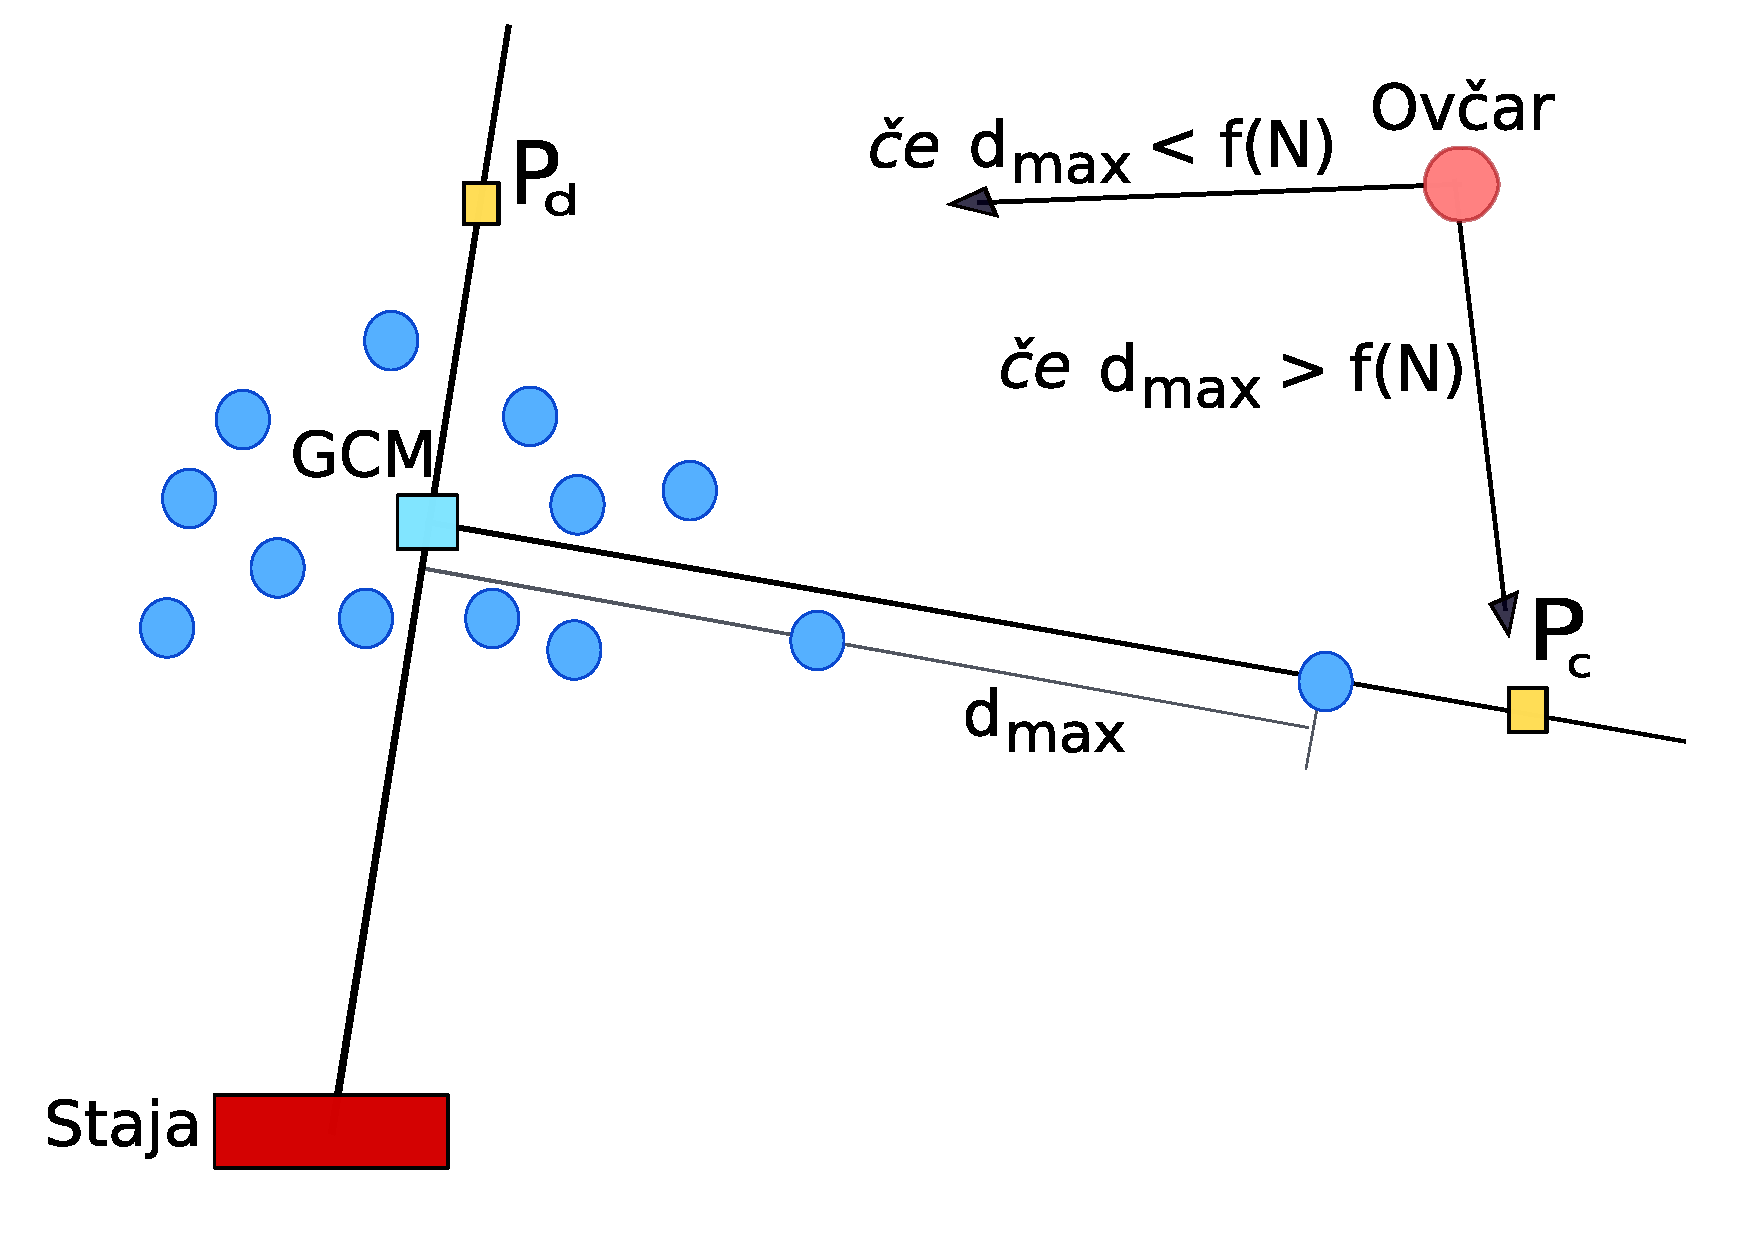
\includegraphics[width=0.8\textwidth]{../poglavja/images/zbiranje.pdf}
	\caption[Stanje zbiranja in vodenja črede]{Ovčar v stanju zbiranja ovc v čredo ali v stanju vodenja črede proti staji.} % narejena je s programom Inkscape
	\label{fig:zbiranje}
\end{figure}

Ko ni nobena ovca več kot $f(N)$ oddaljena od GCM, se ovčar želi postaviti tako, da je čreda oziroma GCM med njim in stajo. Pri tem se postavi $f(N)$ stran od GCM, kot si lahko ogledamo na sliki~\ref{fig:zbiranje}. Temu stanju rečemo stanje vodenja črede. Točko označimo kot $\mathbf{P}_d$.

\subsubsection{Ignoriranje dela črede}

Včasih pa se ovčar znajde v brezizhodni situaciji, ko sam ne obvladuje celotne črede. Zato smo naredili mejo za preklop med zbiranjem in vodenjem bolj ohlapno. Če imamo eno samo pobeglo ovco, je včasih nima smisla pripeljati bliže čredi, ker bi hitreje ostalo čredo privedel do staje in naknadno vanjo pripeljali tudi to ovco. Pobegla ovca je v tem času ogrožena v primeru drugih nevarnosti, ampak v našem primeru ni volkov ali drugih groženj. Ovčar se zato odloči za vodenje črede že v primeru, ko je dovolj velik del črede največ $f(N)$ oddaljen od GCM. Dovoljeni delež pa se spreminja glede na število ovčarjev na sledeč način:
\begin{align}
p = p_z / n_s^{\sigma_s}, \label{eq:ignoriranje}
\end{align}
kjer je $p_z$ utež doslednosti zbiranja, $n_s$ število ovčarjev in $\sigma_s$ moč vpliva velikosti skupine ovčarjev. Več kot je ovčarjev, manj ignoriranih ovc dopuščamo, saj je večja skupina tudi dosti bolj sposobna zbrati veliko čredo. S tem se želimo izogniti možnosti, da bi ovčar ves čas le zbiral čredo, ki bi se mu razpršila vsakič, ko bi šel po ovco, ki jo je izbral, da jo mora pripeljati v čredo.

Pri tem je težava predvsem, da se GCM ne prilagaja vodenemu delu ovc ampak vsem ovcam in se tako lahko prestavi celo tako daleč od črede, da je ovčar ne more več voditi, saj njegove grožnje ne čuti dovolj velik del črede. A to se ne zgodi tako pogosto, sploh pa ne v primeru več ovčarjev, ko je delež ignoriranih ovc tako majhen, da se GCM ne premakne dovolj na račun pobeglih ovc.

\subsubsection{Stanje naključnega premika}

Za primere, ko ovčar ovce pritisne v kot ograde ali pa se pojavi v kakšni drugi ravnovesni situaciji, ki ne dopušča uspeha, smo ovčarju dodali stanje naključnega premika.

V tem stanju si ovčar na vsakih $t_d + U(t_s)$ časovnih enot, kjer je $t_d$ deterministični del in $U(t_s)$ naključni dodatek enakomerno porazdeljen na intervalu $\lbrack 0, t_s\rbrack$, izbere naključno točko na pašniku, proti kateri se premika $t_p$ časovnih enot.

\subsubsection{Stanje premika za čredo}

Ker pa se še vedno lahko zgodi, da se ovčar postavi bliže staji kot GCM, se ovčar v takem primeru premika proti svojemu cilju glede na stanje zbiranja ali vodenja na prilagojen način.

Smer premika izračunamo kot
\begin{align}
\mathbf{s} = \sqrt{\Vert \mathbf{S}_i - \mathbf{F}\Vert}(\mathbf{S}_i - \mathbf{F}) + (\mathbf{P} - \mathbf{S}_i) \sigma_n, \label{eq:zadaj}
\end{align}
kjer je $\mathbf{S}_i - \mathbf{F}$ vektor od staje proti ovčarju, $\mathbf{P} - \mathbf{S}_i$ vektor od ovčarja proti točki $\mathbf{P}_d$ ali $\mathbf{P}_c$, odvisno od zadoščenega pogoja za vodenje ali zbiranje, in $\sigma_n$ utež gibanja za čredo. V primeru, da je ovčar od staje dlje kot GCM, pa se giblje v smeri vektorja od njega proti izbrani točki glede na stanje.

\begin{figure}[ht]  % ali t za na vrhu ali h! za točno tukaj
	\centering
	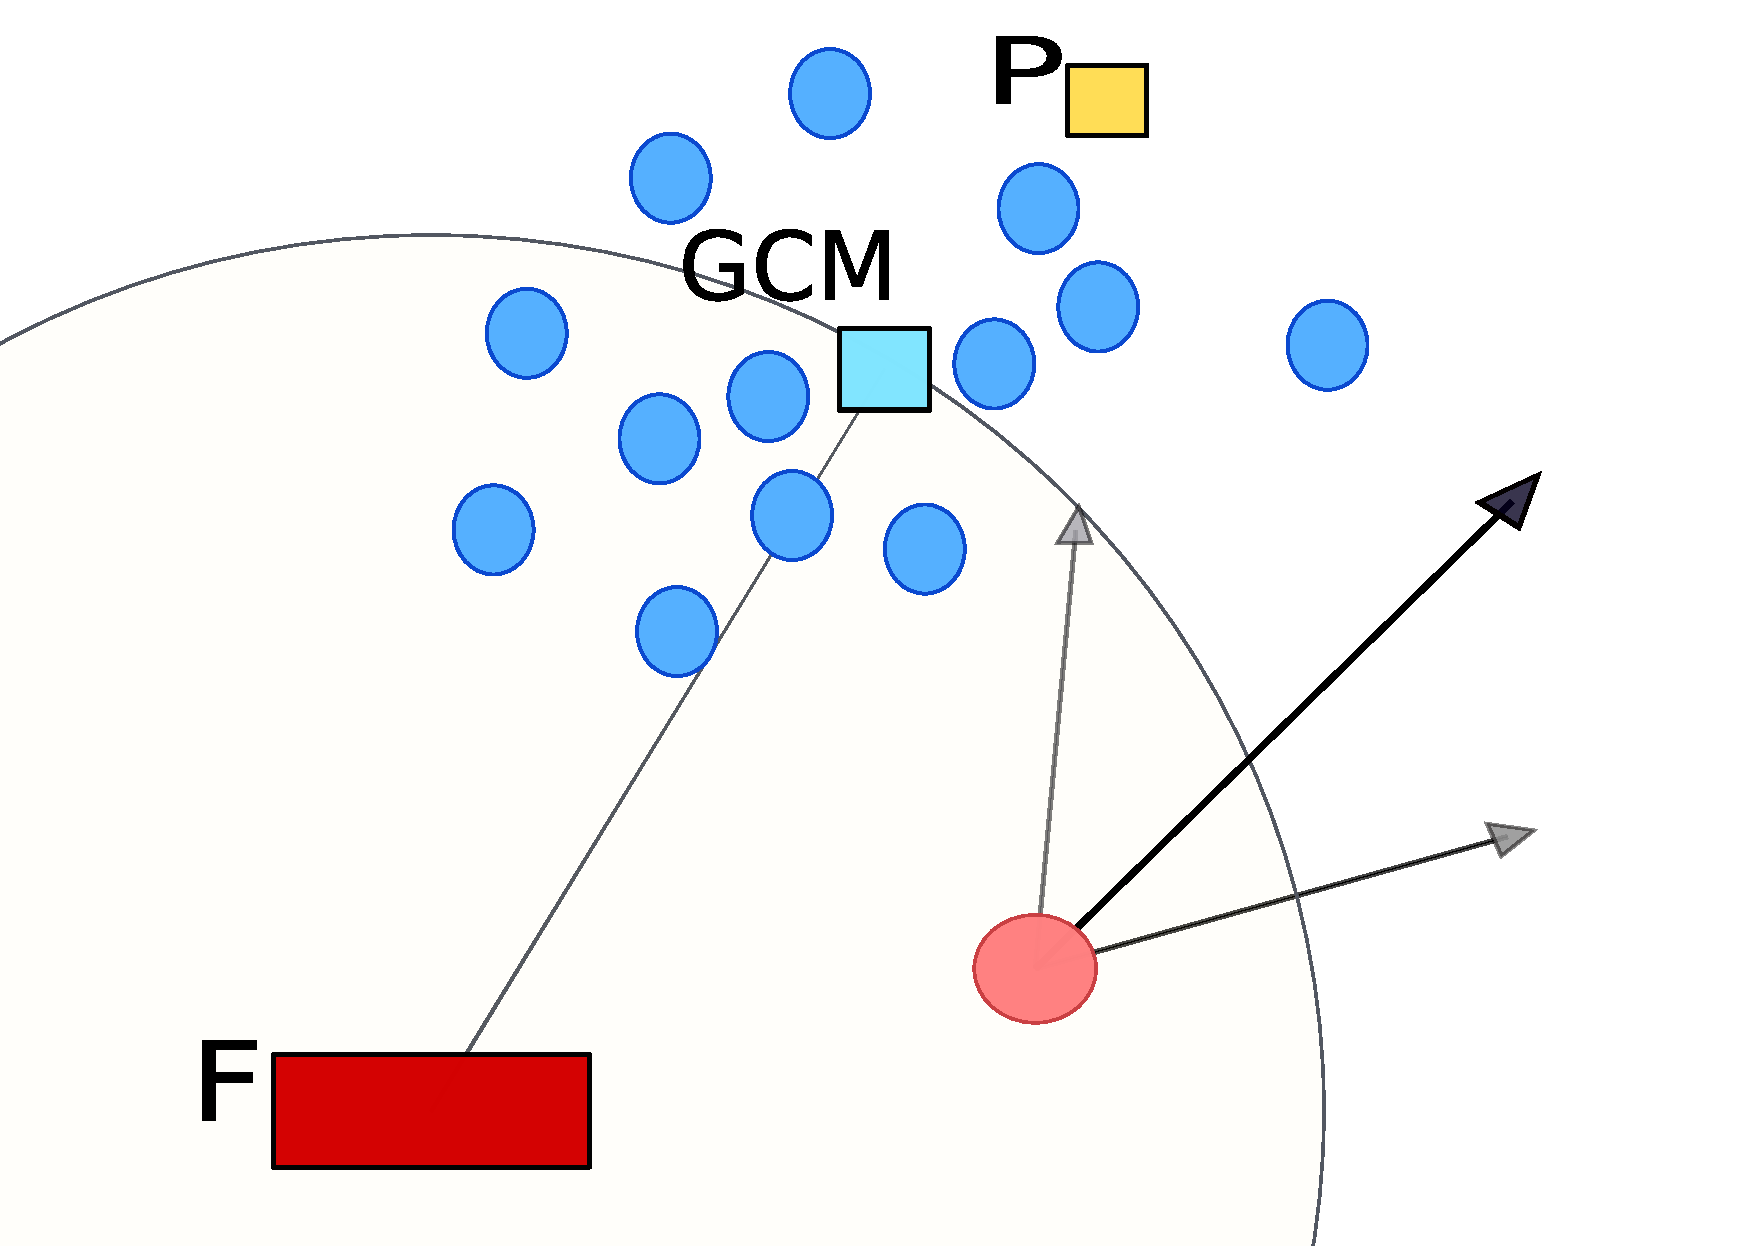
\includegraphics[width=0.49\textwidth]{../poglavja/images/zadaj.pdf}
	\caption[Stanje premika za čredo]{Ovčar v stanju premikanja za čredo.} % narejena je s programom Inkscape
	\label{fig:zadaj}
\end{figure}

\subsubsection{Izbira hitrosti gibanja}

Ovčar ima dve hitrosti med katerima gladko prehaja. Ovčar se premika s hitrostjo vodenja $v_{min}$, kadar je od točke $\mathbf{P}_d$ ali $\mathbf{P}_c$ oddaljen največ $d_t$ in kadar je od njega najbližja ovca oddaljena največ $d_0$. Sicer se giblje s hitrostjo $v_{max}$.

Tako ovčar upočasni v bližini ovc in črede, ker bi jih sicer razkropil, če bi se jim preveč približal.

\subsection{Sodelovanje skupine ovčarjev}\label{sodelovanje}

Ovčar sam pogosto ne more zbrati črede ali pa je pri tem delu zelo neučinkovit, na primer zaradi odsotnosti grožnje, ko gre po pobegle ovce. Tedaj bi bilo dobro, da bi bilo psov več, da si pomagajo in delijo delo. Če ovčarji ne sodelujejo, bodo vedno želeli voditi isto ovco in učinka ne bo. V tem poglavju opišemo način, kako si v našem primeru ovčarji razdelijo delo.

Avtorici članka~\cite{aiba2020suggestion} sta primerjali štiri različne modele sodelovanja dveh psov ovčarjev. Pri tem se modeli razlikujejo v deljenju dela. V prvem modelu je en ovčar ves čas v stanju vodenja in eden v stanju zbiranja, v drugem modelu si vlogi izmenjujeta in nimata nikoli iste vloge, v tretjem največ en ovčar zbira čredo in v četrtem modelu preklapljata med stanjema neodvisno. Pri vseh modelih razen pri prvem si ovčarja čredo delita po premici skozi stajo in skozi GCM. Pri tem se je najbolje izkazal model, kjer sta ovčarja med stanjema neodvisno preklapljala.

Druga možnost poleg deljenja črede bi bila tudi iskanje optimalnih točk, kamor se morajo postaviti ovčarji, in iskanje optimalne poti do teh točk. S tema problemoma se ukvarjajo avtorji člankov~\cite{lee2017autonomous, lien2005shepherding, pierson2015bio, pierson2017controlling}. Mi se bomo pri našem delu osredotočili na delitev črede. Ker si želimo vodenja z večjo skupino psov, moramo najti tudi primerno razdelitev črede na več enot.

Čredo bomo delili na Voronoieve celice z ovčarji v središčih. To pomeni, da ima vsak ovčar svojo Voronoievo celico in v njej vse tiste ovce, ki jim je najbližje izmed vseh ovčarjev. S tem bo vsaka ovca odgovornost le enega ovčarja in ko bo šel ovčar od črede daleč proč po neko ovco, si bodo ostali ovčarji razdelili ostalo čredo. Na sliki~\ref{fig:voronoi} si lahko ogledamo razdelitev črede in dela, kot je opisano v poglavju~\ref{zbiranje}.

\begin{figure}[ht]  % ali t za na vrhu ali h! za točno tukaj
	\centering
	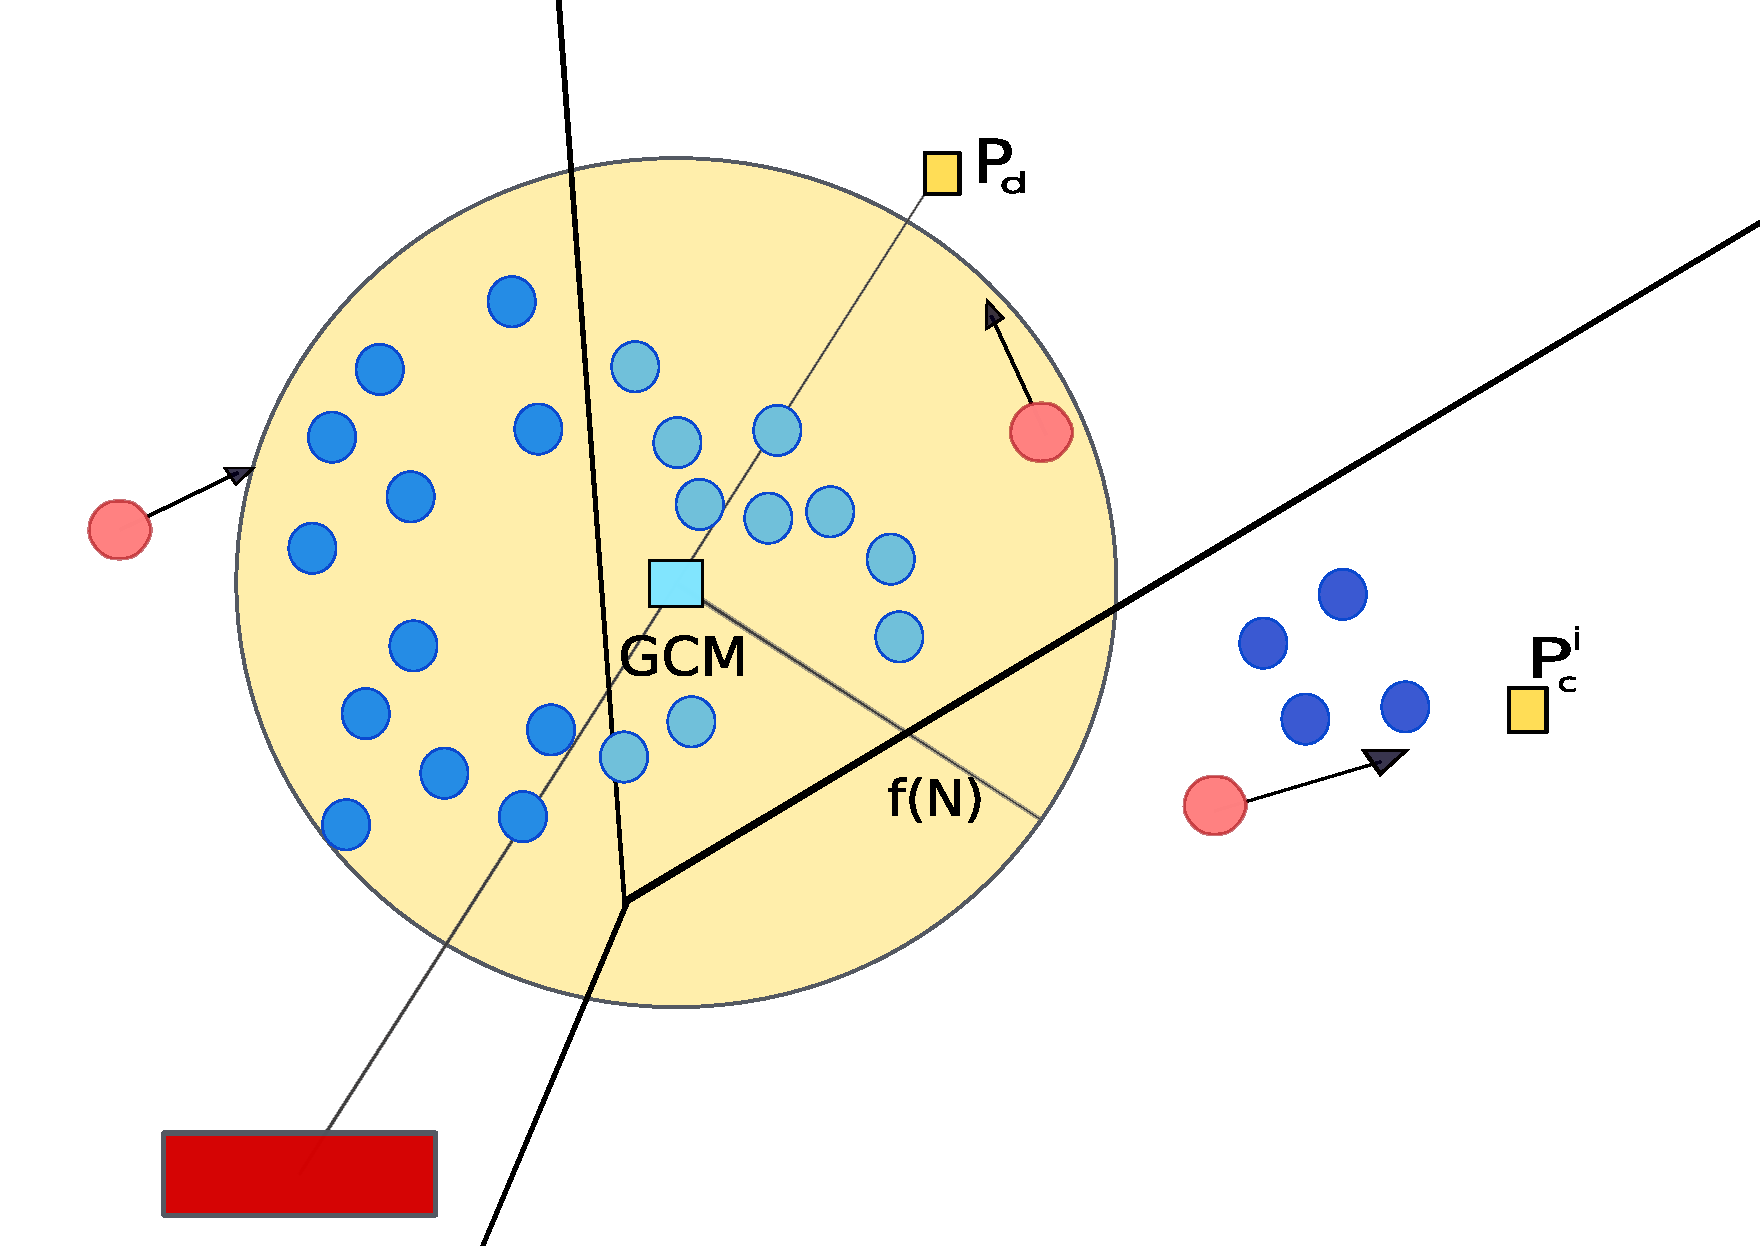
\includegraphics[width=0.9\textwidth]{../poglavja/images/voronoi.pdf}
	\caption[Razdelitev črede in nalog]{Razdelitev črede med tri ovčarje. Dva ovčarja sta v stanju vodenja in en je v stanju zbiranja.} % narejena je s programom Inkscape
	\label{fig:voronoi}
\end{figure}

Ovčarji želijo med seboj ohranjati neko minimalno udobno razdaljo. V ta namen smo med njimi dodali silo odboja z velikostjo $d_s / (r_{ij} + 1)$ v smeri od $j$-tega do $i$-tega ovčarja, ki ga močneje odbija od ovčarjev, ki so mu bliže, kjer je $d_s$ udobna razdalja med ovčarjema in $r_{ij}$ dejanska razdalja med njima povečana za ena v izogib deljenju z majhnim številom. Ker pa ne želimo, da bi se ovčarjem poti križale in želimo njihove poti postaviti bolj vzporedno kot zaporedno, izračunamo tudi kot med njegovo smerjo in lokacijo drugega psa. Njegovi smeri dodamo silo v smeri stran od drugega ovčarja veliko $max(0, sin(\omega))~\sigma_o / (r_{ij} + 1)$, kjer je $\omega$ kot, pod kakršnim gre ovčar proti drugemu ovčarju in je $\sigma_o$ pomen smeri drugih ovčarjev.

\subsection{Premik ovčarja}

Ovčar se torej po zgoraj opisanem načinu giblje glede na stanje obnašanja in hitrost, pri čemer se giblje proti točki trenutnega cilja. Svojo smer pri tem prilagodi glede na prisotnost drugih ovčarjev, na koncu pa njegovo smer še nekoliko popravimo. Dodamo ji šum tako, da jo zasukamo za naključen kot z intervala $\lbrack -e\pi/3, e\pi/3\rbrack$, kjer je $e$ relativna moč šuma. Nato njegovo smer zasukamo za kot $\nu$ stran od ograje, če je tej bliže kot 5~m in se giblje proti njej. Poleg tega njegovo smer zasukamo tudi okrog ovce, če je ta bliže kot $d_a$, ter okrog črede v primeru, da ovčar pride središču črede bliže od $\xi$ deleža razdalje med GCM in točko $\mathbf{P}$ ($\mathbf{P}_c$ ali $\mathbf{P}_d$). Vse tri primere kroženja si lahko ogledamo na sliki~\ref{fig:zaokrozi}. Nato smer zgladimo glede na smer v prejšnjem časovnem koraku. S tem se ovčar giblje bolj naravno.

\begin{figure}[ht]  % ali t za na vrhu ali h! za točno tukaj
	\centering
	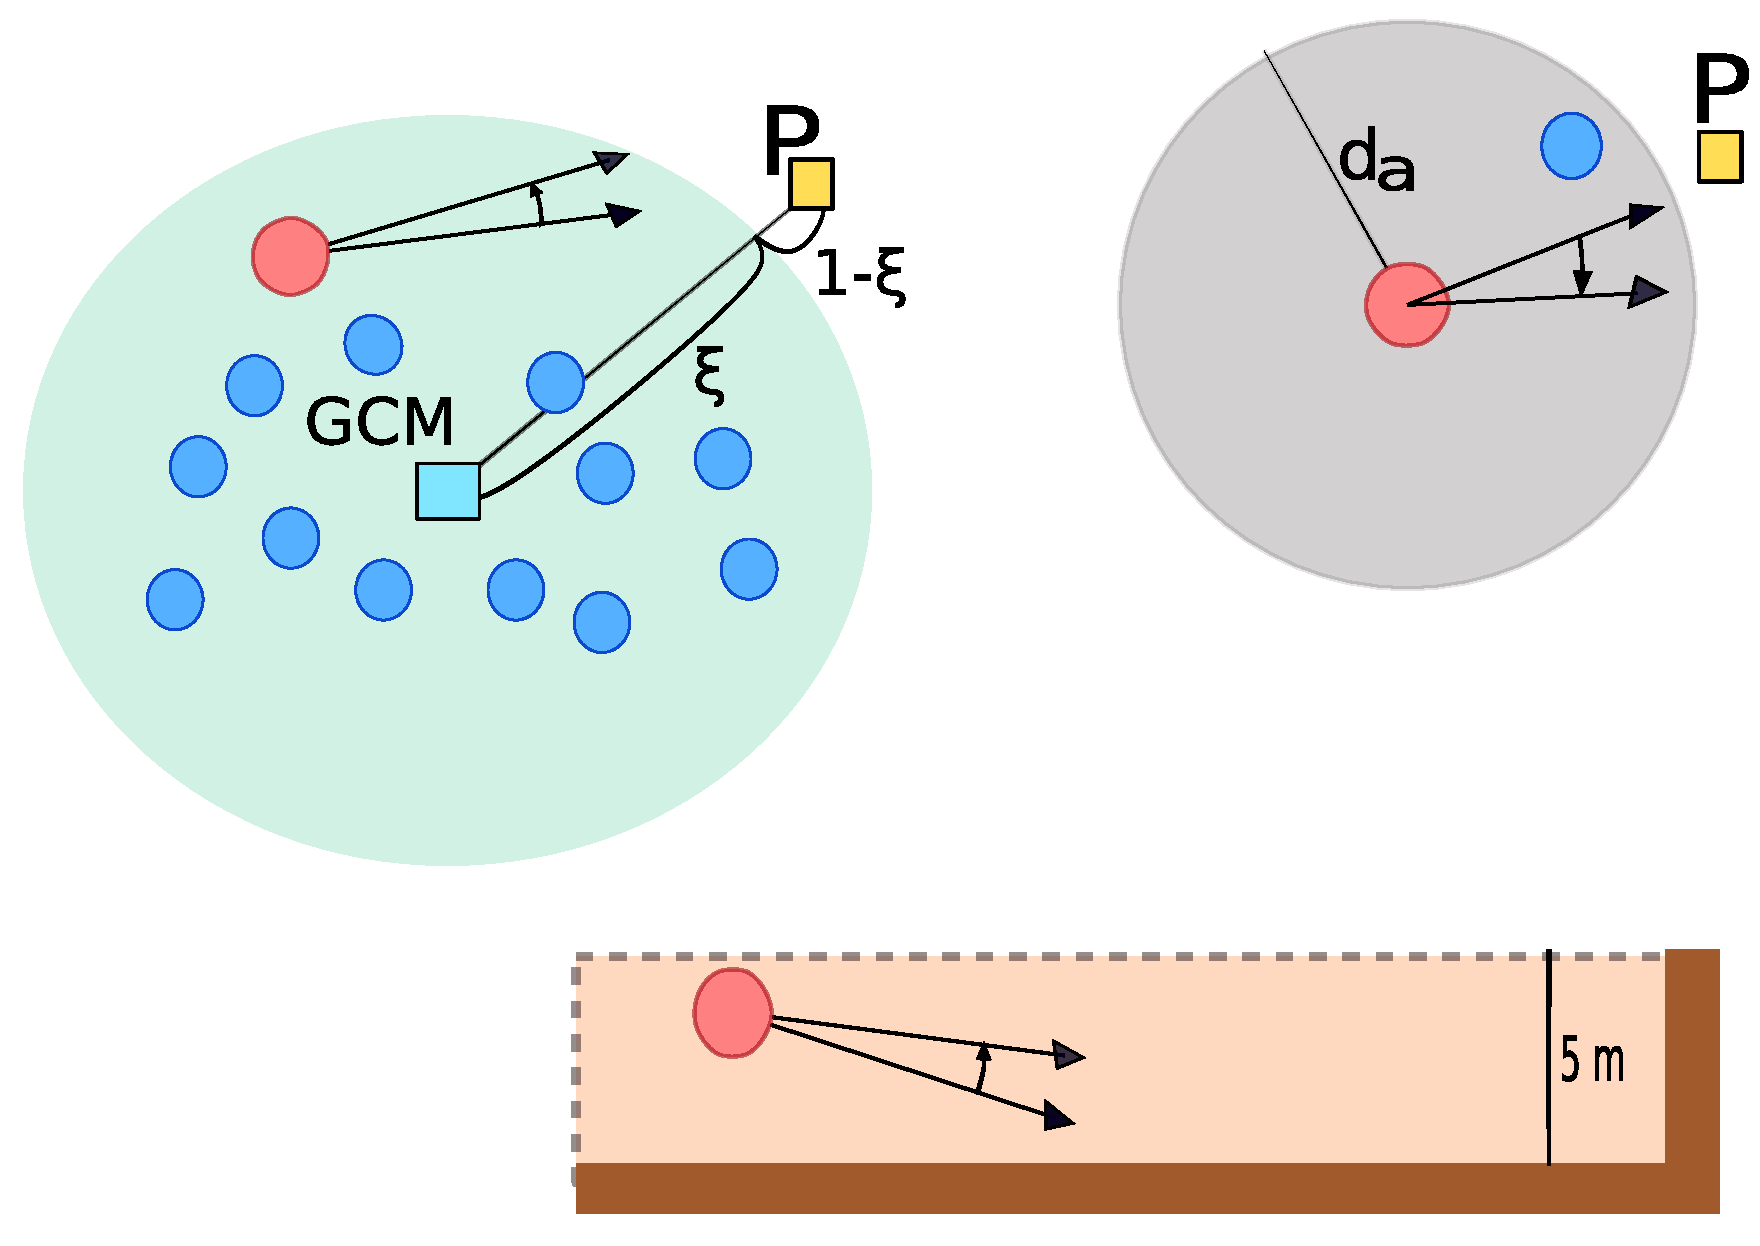
\includegraphics[width=0.9\textwidth]{../poglavja/images/zaokrozi.pdf}
	\caption[Izogibanje ograji, zaokrožanje okrog ovce in okrog črede]{Ovčar zaokroži stran od ograje, ovce ali črede.} % narejena je s programom Inkscape
	\label{fig:zaokrozi}
\end{figure}

V tabeli~\ref{table:ovcar} si lahko ogledamo uporabljene vrednosti parametrov in njihove meje za ostala dva modela.

\begin{table}[ht]
	\begin{center}
		\begin{tabular}{ c|l|c|c }
			\hline
			\textbf{Oznaka} & \textbf{Opis parametra} & \textbf{Vrednost} & \textbf{Interval} \\ \hline  
			$v_{max}$ & Najvišja hitrost & 7,5~m/s & - \\
			$v_{min}$ & Hitrost v stanju vodenja & 5~m/s & $\lbrack 0, v_{max} \rbrack$ \\
			$r_a$ & Faktor za dovoljeno velikost črede & 2~m & $\lbrack 0, 5 \rbrack$ \\
			$d_c$ & Razdalja za zbiranje & 10~m & $\lbrack 0, 30 \rbrack$ \\
			$d_a$ & Razdalja za zaznavo ovc na poti & 20~m & $\lbrack 0, 60 \rbrack$ \\
			$d_0$ & Razdalja za upočasnitve v bližini ovc & 10~m & $\lbrack 0, 30 \rbrack$ \\
			$d_f$ & Razdalja za upočasnitev v bližini cilja & 5~m & $\lbrack 0, 30 \rbrack$ \\
			$e$ & Relativna moč šuma & 30 \% & $\lbrack 0, 50 \rbrack$ \\
			$t_p$ & Trajanje naključnega premika & 3~s & $\lbrack 0, 10 \rbrack$ \\
			$t_d$ & Fiksen čas do naključnega premika & 60~s & $\lbrack 0, 90 \rbrack$ \\
			$t_s$ & Razpon naključnega dodatnega časa & 20~s & $\lbrack 0, 30 \rbrack$ \\
			$\sigma_r$ & Pomen oddaljenosti pobegle ovce od črede & 2 & $\lbrack -1, 4 \rbrack$ \\
			$\sigma_d$ & Pomen oddaljenosti pobegle ovce od ovčarja & 1 & $\lbrack -1, 4 \rbrack$ \\
			$d_b$ & Ovčar bližje cilju kot čreda & 2~m & $\lbrack -5, 50 \rbrack$ \\
			$p_z$ & Največji delež ignoriranih ovc & 15 \% & $\lbrack 0, 40 \rbrack$ \\
			$\sigma_s$ & Vpliv števila ovčarjev na delež ignoriranih ovc & 2 & $\lbrack -1, 4 \rbrack$ \\
			$\sigma_n$ & Odpor pred stanjem bližje cilju kot točka & 2 & $\lbrack 0, 20 \rbrack$ \\
			$d_s$ & Udobna razdalja med ovčarji & 20~m & $\lbrack 0, 40 \rbrack$ \\
			$d_t$ & Razdalja za upočasnitev v bližini točke & 12~m & $\lbrack 0, 20 \rbrack$ \\
			$\xi$ & Odpor pred stanjem pred točko & 95 \% & $\lbrack 0, 1 \rbrack$ \\
			$\nu$ & Zaokroževanje blizu ovc & $\pi / 6$ rad/s & $\lbrack 0, 2 \rbrack$ \\
			$\sigma_o$ & Pomen smeri drugih ovčarjev & 0,1 & $\lbrack -1, 1 \rbrack$ \\
			\hline
		\end{tabular}
	\end{center}
	\caption[Parametri vodenja psa ovčarja]{Parametri psa ovčarja, njihove uporabljene vrednosti za ročno razviti model in njihove meje za ostala dva modela gibanja psa ovčarja. Meje so v istih enotah kot izbrane vrednosti.}
	\label{table:ovcar}
\end{table}
